\section*{Синтез стабилизирующих регуляторов}

\subsection*{Управляемая система 1}

Рассмотрим систему:
\begin{align}
\dot{x}_1 &= -x_1 + 2x_1^3 + x_2 + \sin u_1 \\
\dot{x}_2 &= -x_1 - x_2 + 3\sin u_2
\end{align}

\subsubsection*{Поиск точек равновесия}

При $u_1 = u_2 = 0$ система принимает вид:
\begin{align}
\dot{x}_1 &= -x_1 + 2x_1^3 + x_2 \\
\dot{x}_2 &= -x_1 - x_2
\end{align}

Это система 1, для которой уже найдены точки равновесия:
\begin{itemize}
\item $(0, 0)$ --- устойчивый фокус
\item $(1, -1)$ --- седло
\item $(-1, 1)$ --- седло
\end{itemize}

\subsubsection*{Выбор точки равновесия и линеаризация}

Выберем точку равновесия $(x_1^*,x_2^*) = (0,0)$ и установим стационарные входы $u_{1,ss} = \pi$ (не ноль) и $u_{2,ss} = 0$. Так как $\sin\pi = 0$ и $\sin 0 = 0$, исходные уравнения равновесия совпадают с системой без управления, поэтому $(0,0)$ остаётся точкой равновесия.

Линеаризация проводится по отклонениям $v_1 = u_1 - u_{1,ss}$, $v_2 = u_2 - u_{2,ss}$. Тогда

Матрица $A$:
$$A = \begin{pmatrix} -1 & 1 \\ -1 & -1 \end{pmatrix}$$

Матрица $B = \frac{\partial f}{\partial u}\big|_{ss}$ с учётом $\sin u$:
$$B = \begin{pmatrix} \cos u_{1,ss} & 0 \\ 0 & 3\cos u_{2,ss} \end{pmatrix} = \begin{pmatrix} -1 & 0 \\ 0 & 3 \end{pmatrix}$$

Матрицы весов: $Q = 10I$, $R = I$.

Кратко метод LQR: решаем алгебраическое уравнение Риккати
$$A^T P + PA - PBR^{-1}B^T P + Q = 0,$$
получаем $P$ и вычисляем матрицу обратной связи
$$K = R^{-1}B^T P.$$

Для выбранных $Q=10I$, $R=I$ получено:
$$K = \begin{pmatrix}
-2.2716 & -0.1017 \\
0.3052 & 2.8767
\end{pmatrix},$$

собственные значения $A - BK$:
$$\sigma(A-BK) = \{-3.5548,\;-9.3468\},$$
что указывает на локальную экспоненциальную устойчивость. Нелинейные моделирования подтверждают стабилизацию.


\subsection*{Управляемая система 2}

Рассмотрим систему:
\begin{align}
\dot{x}_1 &= x_2 + x_1 x_2 + u \\
\dot{x}_2 &= -x_2 + x_2^2 - x_1^3 + \sin u
\end{align}

\subsubsection*{Поиск точек равновесия}

При $u = 0$ система принимает вид:
\begin{align}
\dot{x}_1 &= x_2 + x_1 x_2 \\
\dot{x}_2 &= -x_2 + x_2^2 - x_1^3
\end{align}

Точки равновесия находятся из решения:
\begin{align}
x_2(1 + x_1) &= 0 \\
-x_2 + x_2^2 - x_1^3 &= 0
\end{align}

\textbf{Случай 1:} $x_2 = 0$. Из второго уравнения: $-x_1^3 = 0 \Rightarrow x_1 = 0$

\textbf{Случай 2:} $x_1 = -1$. Из второго уравнения: $-x_2 + x_2^2 - (-1)^3 = 0 \Rightarrow x_2^2 - x_2 + 1 = 0$

Дискриминант: $D = 1 - 4 = -3 < 0$ --- нет действительных решений.

\textbf{Точка равновесия:} $(0, 0)$

\subsubsection*{Выбор точки равновесия и линеаризация}

Выберем точку равновесия $(x_1^*,x_2^*) = (0,0)$ и установим стационарный вход $u_{ss} = 0$.

Линеаризация по отклонению $v = u - u_{ss}$:

Матрица $A$:
$$A = \begin{pmatrix} 0 & 1 \\ 0 & -1 \end{pmatrix}$$

Матрица $B = \frac{\partial f}{\partial u}\big|_{ss}$ с учётом $\sin u$ в $\dot x_2$:
$$B = \begin{pmatrix} 1 \\ 1 + \cos u_{ss} \end{pmatrix} = \begin{pmatrix} 1 \\ 2 \end{pmatrix}$$

Матрицы весов: $Q = 10I$, $R = 1$.

Кратко метод LQR: решаем уравнение Риккати $A^T P + PA - PBR^{-1}B^T P + Q = 0$ и вычисляем $K = R^{-1}B^T P$.

Для $Q=10I$, $R=1$ получено:
$$K = \begin{pmatrix} 3.1623 & 2.1014 \end{pmatrix},$$
собственные значения $A-BK$:
$$\sigma(A-BK) = \{-1.3529,\;-7.0121\},$$
что обеспечивает локальную экспоненциальную устойчивость в выбранной точке. Моделирование подтверждает стабилизацию.

\subsection*{Численное моделирование}

Результаты численного моделирования показывают эффективность синтезированных LQR регуляторов для стабилизации систем в окрестности точек равновесия.

\begin{figure}[H]
\centering
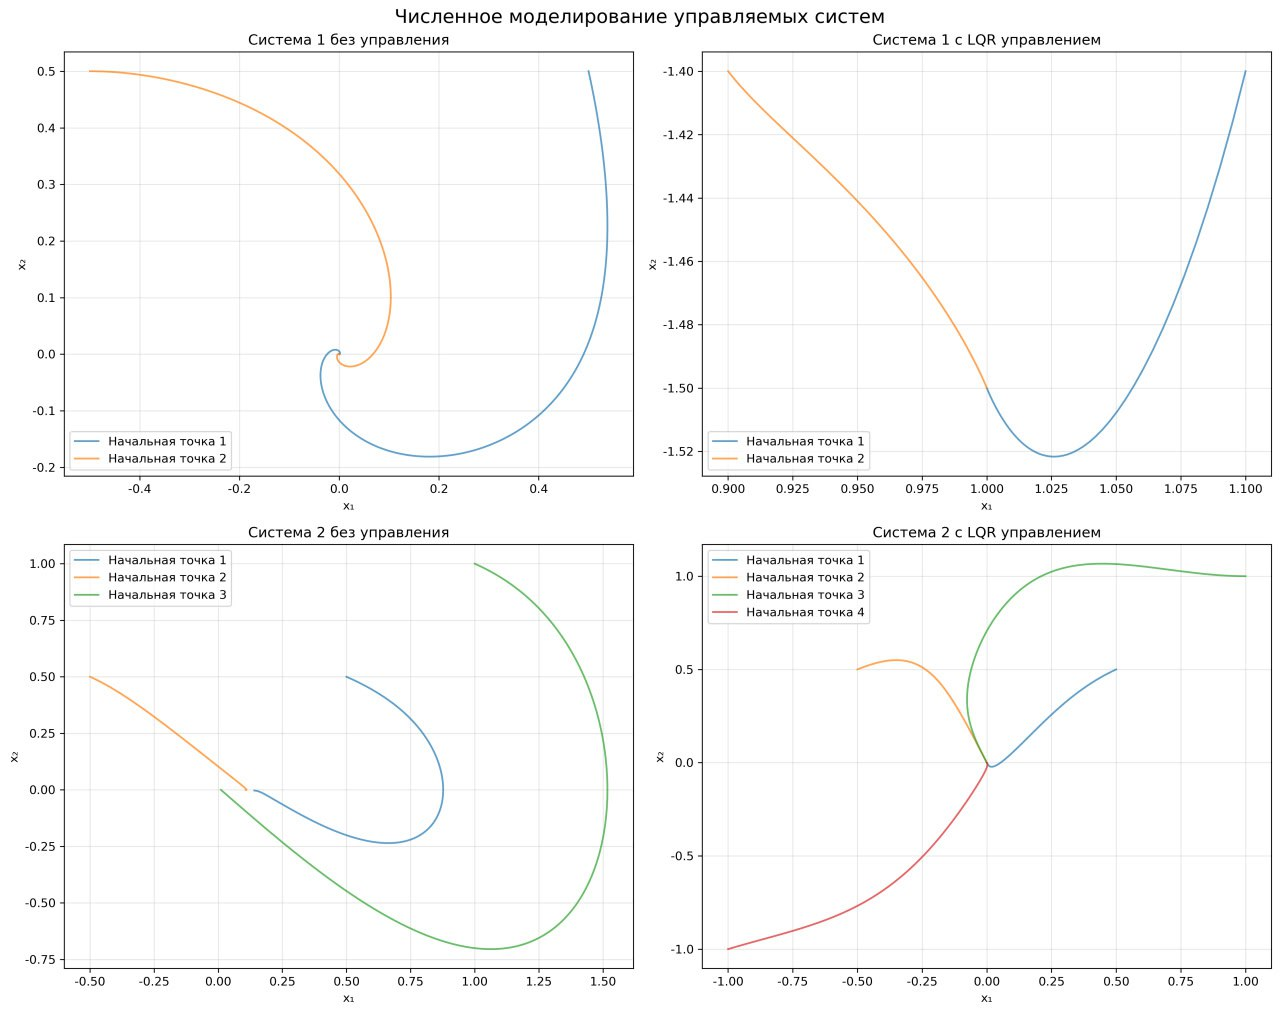
\includegraphics[width=0.8\textwidth]{controlled_systems/controller_simulation.png}
\caption{Результаты численного моделирования управляемых систем}
\label{fig:controller_sim}
\end{figure}
